\documentclass[USenglish,oneside,twocolumn]{article}

\usepackage[utf8]{inputenc}%(only for the pdftex engine)
%\RequirePackage[no-math]{fontspec}%(only for the luatex or the xetex engine)
\usepackage[big]{dgruyter_NEW}

%%%%
% Paul's preprint settings (1/2)
%%%
%\usepackage{fancyhdr}
%\renewcommand{\headrulewidth}{0pt}
%\lhead{}
%\rhead{}
%\cfoot{DISTRIBUTION A:  Approved for public release, distribution is unlimited}


% allow URL breaks on dashes
\def\UrlBreaks{\do\/\do-}

% math environment
\usepackage{mathtools}
\usepackage{amsmath}
\usepackage{amssymb}
\usepackage[%
    lambda, advantage, operators, sets, adversary, landau, probability, notions,
    logic, ff, mm, primitives, events, complexity, asymptotics, keys,
]{cryptocode}

% prettier line breaks
\usepackage{microtype}

% figures
\usepackage{graphicx}
\usepackage[position=bottom]{subfig}
\usepackage{tikz}
\usepackage{tikz-qtree}
\usetikzlibrary{shapes.misc,positioning,arrows,snakes,calc}

% colors
\usepackage{color}
\usepackage{colortbl}
\definecolor{rgddTeal}{HTML}{009999}
\definecolor{rgddLime}{HTML}{809933}
\definecolor{rgddPurple}{HTML}{993380}
\definecolor{rgddDred}{HTML}{E04644}
\definecolor{rgddDgreen}{HTML}{008000}
\definecolor{rgddDblue}{HTML}{2809B2}

% custom commands
\newcommand{\TODO}[1]{\textcolor{red}{TODO:} \emph{#1}}

 
\DOI{foobar}

\cclogo{
\includegraphics{by-nc-nd.pdf}}
  
\begin{document}
  \author*[1]{Corresponding Author}
  \author[2]{Second Author}
  \author[3]{Third Author}
  \author[4]{Fourth Author}
  \affil[1]{Affil, E-mail: email@email.edu}
  \affil[2]{Affil, E-mail: email@email.edu}
  \affil[3]{Affil, E-mail: email@email.edu}
  \affil[4]{Affil, E-mail: email@email.edu}

% \author*[1]{Rasmus Dahlberg}
% \author[2]{Tobias Pulls}
% \author[3]{Tom Ritter}
% \author[4]{Paul Syverson}
% \affil[1]{Karlstad University, E-mail: rasmus.dahlberg@kau.se}
% \affil[2]{Karlstad University, E-mail: tobias.pullsg@kau.se}
% \affil[3]{Mozilla, E-mail: tom@ritter.vg}
% \affil[4]{U.S. Naval Research Laboratory, E-mail: paul.syverson@nrl.navy.mil}


  \title{\huge%
  Privacy-Preserving \& Incrementally-Deployable Support for Certificate Transparency in Tor
  }
  \runningtitle{%
	Privacy-Preserving \& Incrementally-Deployable Support for Certificate Transparency in Tor
  }
  %\subtitle{...}

  \begin{abstract}
      {The security of the web has greatly improved in the last couple of years. HTTPS
is now the default, with browsers moving towards warning when unencrypted
connections are made. The Certificate Authority (CA) system has also improved.
The advent of mandatory Certificate Transparency (CT) logging of all
certificates issued by CAs---enforced by web browsers---has made the
weakest-link setting of the CA system more sustainable. However, Tor and its Tor
Browser, based on Firefox, is missing support for CT.

In this paper, we present designs for privacy preserving and
incrementally-deployable support for CT in Tor. Our designs go beyond
the support for CT found in browsers like Google Chrome or Apple's
Safari: we aim to do more than detect CA misbehavior supporting
man-in-the-middle or impersonated HTTPS connections from Tor Browser.
We also create independent public evidence of CT log misbehavior in
support of this. Our base design shares observed certificates in Tor
Browser with other CT logs. Associated privacy leaks of browsing
behavior of Tor users are minimized through the use of indirect
routing and randomized delay of certificate reporting through relays
in the Tor network.

We also present two possible extensions to our base design that can also detect
CT log misbehavior. One extension makes a slight change to the API and operation
of CT logs, the other adds more complexity to Tor but in turn completely removes
all trust placed in CT log operators. Detecting CT log misbehavior is
particularly important for the wider web, since CT as currently deployed lacks
strong mechanisms necessary for reducing trust in CT log operators.
We turn Tor into a system for maintaining a probabilistically-verified view of
the CT log ecosystem as available from Tor’s consensus.
}
  \end{abstract}

  \keywords{Certificate Transparency, Tor}
  %\classification[PACS]{}
  %\communicated{...}
  %\dedication{...}

  \journalname{Proceedings on Privacy Enhancing Technologies}
  \DOI{Editor to enter DOI}
  \startpage{1}
  \received{..}
  \revised{..}
  \accepted{..}

  \journalyear{..}
  \journalvolume{..}
  \journalissue{..}
 
  \maketitle
  %%%%
  % Paul's preprint settings (1/2)
  %%%
  %\pagestyle{fancy}
  %\thispagestyle{fancy}

  \section{Introduction} \label{sec:introduction}
Metrics reported by Google and Mozilla reveal that encryption on the web
skyrocketed the past couple of years: at least 85\% of all web pages load using
Transport Layer Security (TLS) as part of
HTTPS~\cite{google-metrics,mozilla-metrics}. An HTTPS connection is initiated by
a TLS handshake where the client web browser requires that the web server
presents a valid certificate to authenticate the identity of the server (e.g.,
to make sure that the client who wants to visit \url{mozilla.org} really is
connecting to Mozilla, and not, say, Google). A certificate is considered valid
if it is digitally signed by a Certificate Authority (CA) that the browser
trusts. Each CA is trusted to certify (sign) that specific cryptographic
key-material as part of a certificate belongs to a particular domain name.

The CA trust model suffers from \emph{weakest-link} security: web browsers trust
hundreds of CAs, and it is enough to compromise a single CA to get a certificate
mis-issued in the name of a target domain~\cite{ca-ecosystem,https-sok}.
Motivated by this issue manifested by prominent CA compromises---such as the
issuance of a fraudulent certificate for \url{google.com} by DigiNotar in
2011\footnote{\url{https://web.archive.org/web/20200521135444/https://arstechnica.com/information-technology/2011/08/earlier-this-year-an-iranian/}}---several
major browser vendors have mandated that certificates issued by CAs must be
included into trusted Certificate Transparency (CT) logs for browsers to trust
them~\cite{ct/a,ct,ct/bis}. The idea behind CT is that, by making all issued
certificates transparent, mis-issued certificates can be detected \emph{after}
issuance and appropriate actions taken to keep the wider web safe (e.g.,
revocation of certificates, suspected compromises investigated, or trust in
misbehaving CAs removed from browsers). Browsers that wish to benefit from CT
augment the validation done by the browser during the TLS handshake to also
require cryptographic proof from the server that the presented certificate has
been included into CT logs trusted by the browser. Notable browsers with
mandatory CT support by default are Google Chrome and Apple's Safari
\cite{chrome-policy,safari-policy}. Unfortunately, Mozilla's Firefox lacks
support but has a partial implementation.

Beyond security on the web, anonymous access to the web has also matured. In
particular, Tor with its Tor Browser (TB) today have millions of daily users
\cite{tor,mani}, and effort is ongoing into maturing the technology for wider
use\footnote{\url{https://web.archive.org/web/20200528174708/https://mozilla-research.forms.fm/mozilla-research-grants-2019h1/forms/6510}}.
The basis of TB is Firefox, where TB then enables anyone to browse the web
anonymously by relaying traffic between browser and web server through the Tor
network, consisting of thousands of voluntary-run relays across the globe. 

Just like attackers may be interested in breaking HTTPS, attackers are
interested in breaking the anonymity provided by Tor with the goal of
deanonymizing users. One common deanonymization technique, known to be used in
practice by, e.g., law enforcement, is to compromise TB instead of directly
circumventing the anonymity provided by the Tor
network\footnote{\url{https://web.archive.org/web/20200528175225/https://zerodium.com/tor.html}}.
Modern web browsers like TB (Firefox) are one of the most complex types of
software in wide use today. This complexity and wide use leads to security
vulnerabilities and incentives for exploitation. For example, the exploit
acquisition platform Zerodium offers up to \$100,000 for a zero-day exploit
against Firefox that leads to remote code execution and local privilege
escalation\footnote{\url{https://web.archive.org/web/20200521151311/https://zerodium.com/program.html}}
(i.e., full control of the browser for the attacker).

An attacker that wishes to use such an exploit to compromise and then ultimately
deanonymize a TB user has to deliver the exploit to TB\@. Since the web is
mostly encrypted today, this primarily has to happen over an HTTPS connection,
where the attacker controls the content returned by the web server. While there
are a number of possible ways for an attacker to accomplish this (e.g., by
compromising a web server that the target TB user connects to), one option is to
\emph{impersonate} a web server by acquiring a fraudulent certificate. Due to
the Tor network being run by volunteers, getting into a position for performing
such an attack is relatively straightforward (the attacker can volunteer to run
malicious relays~\cite{spoiled-onions}). The same is true for an attacker that
wishes to \emph{man-in-the-middle} connections made by TB users. In such a case,
a TB exploit may not even be needed to deanonymize the user; e.g., if the user
logs into an account at the service associated with its identity and that the
attacker can now observe.

\subsection{Introducing CTor}
In this paper, we propose an incremental design which we refer to as CTor. CTor
brings CT to Tor by modifying both how TB and relays in the Tor network work.
The goal is to make impersonation and man-in-the-middle attacks on HTTPS
connections \emph{detectable after the fact} when they are carried out by a
powerful attacker that:
\begin{itemize}
	\item can acquire a forged certificate from a trusted CA,
	\item with the necessary forged cryptographic proofs from CT logs so that TB
	accepts the certificate as valid (with no intent of making the forged
	certificate publicly available in a CT log), and
	\item has the capability to fully gain control of TB shortly after the
	establishment of the HTTPS connection.
\end{itemize}

Our base CTor design uses the CT log ecosystem against the attacker to ensure a
non-zero (tweakable) probability of detection of the forged certificate. This is
done by probabilistically adding the certificate to \emph{other CT logs} than
those directly inferable as under attacker control (due to the accompanying
proofs). TB uses modified relays to cache and interact with CT logs for the sake
of privacy, ensuring that CT log operators (such as Google and Cloudflare) do
not get a real-time feed of all browsing activities from TB (beyond what their
privileged position on the Internet already provides them~\cite{TorDNS}). 
% FIXME: some other source would be good above, have to mention DNS to make
% current one make sense

Beyond the base CTor design we present two extensions. Both extensions have in
common that their goal is to make transparent the forged cryptographic proofs
from attacker-controlled CT logs used to get TB to accept malicious HTTPS
connections. Such a proof would likely immediately disqualify each offending CT
log and thus come and great cost to the attacker in terms of lost capability.
Even a small probability of detection may entail unacceptable risk at such a
high cost. Note that we have already observed several instances of CT logs that
misbehaved~\cite{izenpe-disqualified,venafi-disqualified,gdca1-omission}. Most
recently, a compromised CT log signing key was reported for the first
time~\cite{digicert-log-compromised}. 

The key change in the first extension is that relays now challenge CT logs to
cryptographically prove the correctness of their prior proofs presented to TB
instead of simply sharing the certificates (the subject of the proofs) with
other CT logs. In case an offending CT log fails to provide such a proof
in a timely manner,
the querying relay ensures that the proof arrives at a trusted auditor. While
this adds both more complexity and operational challenges to Tor (of both
auditors and storage at relays), it completely removes all trust in the CT
ecosystem. Another benefit is that, as a consequence of CTor's design, Tor would
provide a probabilistically-audited cryptographically-verifiable view of the
entire CT log ecosystem. This significantly addresses one of the main open
issues with the currently deployed CT ecosystem: the lack of a sufficiently
secure gossiping mechanism that makes it possible to place zero-trust in the log
operators.

The second extension involves only a minor tweak to the base CTor design.
Unfortunately, this tweak is primarily not to Tor but to the API of CT logs.
While similar changes have been discussed earlier in the context of gossiping in
CT, it is a significant deployment issue. The small tweak is that CT logs
provide an API for receiving cryptographic proofs made by other CT logs wrt
certificate inclusion. This would then mean that relays would add to
other CT logs proofs observed by TB clients in addition to the certificate.
This would also significantly reduce the trust assumptions the wider web has to
place on CT log operators, from close to full trust as-is today to only trusting
that some operators are honest.

\subsection{Contribution and Structure}
Section~\ref{sec:background} provides necessary background on CT and Tor. Our
threat model is described in detail in Section~\ref{sec:adversary}, taking into
account the threat models of both Tor and CT\@.

Section~\ref{sec:base} presents the base design of CTor that enables TB to
probabilistically provide evidence to CT logs that it has been presented with a
fraudulent certificate. This greatly impacts risk-averse attackers, since part
of its fraudulent behavior has been made transparent through the CT ecosystem:
the issuing CA may get revoked from the trust store of browsers, the domain name
in question (as part of the certificate) is made public, and awareness of the
event may draw unwanted attention. Our security analysis, in
Section~\ref{sec:analysis}, shows that one of the best bets for an attacker may
be to attack the entire Tor network: an act that in itself may draw unwanted
attention.

Two extensions to the base CTor design are presented in
Sections~\ref{sec:auditor} and \ref{sec:log}. Both extensions aim to make
transparent the accompanying fraudulent proofs issued by CT logs to convince TB
to accept a fraudulent certificate. The deployment of either design would
greatly contribute to the open question of how to reduce trust in CT log operators
currently caused by the lack of an appropriate gossiping mechanism~\cite{FIXME}.
In particular, the auditor-based design (Section~\ref{sec:auditor}) would result
in a probabilistically-audited cryptographically-verifiable view of the entire
CT log ecosystem available from Tor's consensus. This view could be used as the
basis for trust by other browsers, greatly improving the security posture of the
entire web.

Section~\ref{sec:performance} estimates performance aspects of our designs,
including estimated circuit overhead and estimated load on the Tor network.
Privacy aspects of our design choices are covered in Section~\ref{sec:privacy},
with a focus on the essential role of the distributed nature of the Tor network
in both preserving privacy of Tor users as well as the overall security of our
proposed designs. In gist, a similar approach would not work without Tor, e.g.,
if integrated into Google Chrome. Finally, Section~\ref{sec:related} covers
related work and Section~\ref{sec:conclusion} concludes this paper.

%%% Local Variables: 
%%% mode: latex 
%%% TeX-master: "../main"
%%% End:          

  \section{Background} \label{sec:background}
The theory and current practise of CT is introduced first, then Tor
and its privacy-preserving Tor Browser.

\subsection{Certificate Transparency} \label{sec:background:ct}
The idea to transparently log TLS certificates emerged at Google in response to
a lack of proposals that could be deployed without drastic ecosystem changes
and/or significant downsides~\cite{ct/a}.  By making the set of issued
certificate chains\footnote{%
	A domain owner's certificate is signed by an intermediate CA, whose
	certificate is in turned signed by a root CA that acts as a trust
	anchor~\cite{ca-ecosystem}.  Such a \emph{certificate chain} is valid if it
	ends in a trusted anchor that is shipped in the user's system software.
} transparent, anyone that inspect the logs can detect certificate
mis-issuance \emph{after the fact}.  It would be somewhat circular to solve
issues in the CA ecosystem by adding trusted CT logs.  Therefore, the
cryptographic foundation of CT is engineered to avoid any such reliance.
Google's \emph{gradual} CT rollout started in 2015, and evolved from merely
downgrading user-interface indicators in Chrome to the current state of hard
failures unless a certificate is accompanied by a signed \emph{promise} that it
will appear in two independent CT logs~\cite{does-ct-break-the-web}.  Unlike
Apple's CT enforcement~\cite{safari-policy}, one of these logs must additionally
be operated by Google~\cite{chrome-policy}.

The lack of mainstream verification, i.e., beyond checking signatures, allows an
attacker to side-step the current CT enforcement with minimal risk of exposure
\emph{if the required logs are controlled by the attacker}.  
CTor integrates into the gradual CT roll-out by starting on the same
premise of pairwise-independently trusted logs, which
avoids the risk of bad user experience~\cite{does-ct-break-the-web}
and significant system complexity.  For example, web pages are unlikely to
break, TLS handshake latency stays about the same, and no robust management of
suspected log misbehavior is needed.  Retaining the latter property as part of
our incremental designs simplifies deployment.

\subsubsection{Cryptographic Foundation}
The operator of a CT log maintains a tamper-evident append-only Merkle
tree~\cite{ct,ct/bis}.  At any time, a Signed Tree Head (STH) can be produced
which fixes the log's structure and content.  Important attributes of an STH
include
	the tree head (a cryptographic hash),
	the tree size (a number of entries), and
	the current time.
Given two tree sizes, a log can produce a \emph{consistency proof} that proves
the newer tree head entails everything that the older tree head does.  As such,
anyone can verify that the log is append-only without downloading all entries
and recomputing the tree head.  Membership of an entry can also be proven
by producing an \emph{inclusion proof} for an STH.  These proof techniques are
formally verified~\cite{secure-logging-and-ct}.

Upon a valid request, a log must add an entry and produce a new STH that covers
it within a time known as the Maximum Merge Delay (MMD), e.g., 24~hours.  This
policy aspect can be verified because in response, a Signed Certificate
Timestamp (SCT) is returned.  An SCT is a signed promise that an entry will
appear in the log within an MMD.  A log that violates its MMD is said to perform
an \emph{omission attack}.  It can be detected by challenging the log to prove
inclusion.  A log that forks, presenting one append-only version
to some entities and another to others, is said to perform a \emph{split-view
attack}.  Split-views can be detected by STH
gossip~\cite{chuat,dahlberg,nordberg,syta}.

\subsubsection{Standardization and Verification}
The standardized CT protocol defines public HTTP(S) endpoints that allow anyone
to check the log's accepted trust anchors and added certificates, as well as
to obtain the most recent STH and to fetch proofs~\cite{ct,ct/bis}.  For
example, the \texttt{add-chain} endpoint returns an SCT if the added certificate
chain ends in a trust anchor returned by the \texttt{get-roots} endpoint.  We
use \texttt{add-chain} in Section~\ref{sec:incremental}, as well as several
other endpoints in Section~\ref{sec:base} to fetch proofs and STHs.  It might be
helpful to know that an inclusion proof is fetched based on two parameters: a
certificte hash and the tree size of an STH.  The former specifies the log entry
of interest, and the latter with regards to which view inclusion should be
proven.  The returned proof is valid if it can be used in combined with the
certificate to reconstruct the STH's tree head.

The CT landscape provides limited value unless it is verified that the logs
play by the rules.  The rules are influenced by the major browser vendors that
define \emph{CT policies}.  For example, how is CT enforced by their user
agents, and what is required to become a recognized CT log in terms of uptime
requirements and accepted trust anchors.  Google Chrome and Apple's Safari
require that a certificate chain must be accompanied by two independent
SCTs~\cite{chrome-policy,safari-policy}, where independence refers to the
associated log operators.  While there are several ways that a log can misbehave
with regards to these policy aspects, the most fundamental forms of cheating are
omission and split-view attacks.  A party that follows-up on inclusion and
consistency proofs is said to \emph{audit} the logs.

Widespread client-side auditing is a premise for CT logs to be untrusted, but
none of the web browsers that enforce CT engage in such activities yet.  For
example, requesting an inclusion proof is privacy-invasive because it leaks
browsing patterns to the logs, and reporting suspected log misbehavior comes
with privacy~\cite{ct-with-privacy} as well as operational challenges.
Found log incidents are mostly reported manually to the CT policy
list~\cite{ct-policy-mailing-list}.  This is in contrast to automated
\emph{CT monitors}, which notify domain owners
of newly issued certificates based on what actually appeared in the public
logs~\cite{lwm,ct-monitors}.

\subsection{Tor} \label{sec:background:tor}

Most of the activity of Tor's millions of daily users starts with Tor Browser
and connects to some ordinary website via a circuit comprised of three
randomly-selected Tor relays. In this way no identifying information from
Internet protocols (such as IP address) are automatically provided to the
destination, and no single entity can observe both the source and destination of
a connection. Tor Browser is also configured and performs some filtering to resist
browser fingerprinting, and first party isolation to resist sharing state or
linking of identifiers across origins. More generally it avoids storing
identifying configuration and behavioral information to disk.

Tor relays in a circuit are selected at random, but not uniformly. A typical
circuit is comprised of a \emph{guard}, a \emph{middle}, and an \emph{exit}. A
guard is selected by a client and used for several months as the entrance to all
Tor circuits. If the guard is not controlled by an adversary, that adversary
will not find itself selected to be on a Tor circuit adjacent to (thus
identifying) the client. And because some relay operators do not wish to act as
the apparent Internet source for connections to arbitrary destinations, relay
operators can configure the ports (if any) on which they will permit connections
besides to other Tor relays. Finally, to facilitate load balancing, relays are
assigned a weight based on their apparent capacity to carry traffic. In keeping
with avoiding storing of linkable state, even circuits that share an origin will
only permit new connections over that circuit for ten minutes. After that, if
all connections are closed, all state associated with the circuit is cleared.
Similarly, at each relay state associated with a given circuit is cleared
shortly after a circuit is closed.

Tor clients use this information when choosing relays with which to build a
circuit. They receive the information via an hourly updated \emph{consensus}.
The consensus assigns weights as well as flags such as \texttt{guard} or
\texttt{exit}. It also assigns auxiliary flags such as
\texttt{stable}, which, e.g.,
is necessary to obtain the \texttt{guard} flag since guards must have good
availability. Self-reported information by relays in their \emph{extra-info
document}, such as statistics on their read and written bytes, are also part of
the consensus and uploaded to \emph{directory authorities}. Directory
authorities determine the consensus by voting on various components making up
the shared view of the state of the Tor network. Making sure that all clients
have a consistent view of the network prevents epistemic attacks wherein clients
can be separated based on the routes that are consistent with their
understanding~\cite{danezis:pets2008}. This is only a very rough sketch of Tor's
design and operation.  More details can be found by following links at Tor's
documentation site~\cite{tor-documentation}.

Tor does not aim to prevent end-to-end correlation attacks. An adversary
controlling the guard and exit, or controlling the destination and observing the
client ISP, etc. is assumed able to confirm who is connected to whom on that
particular circuit. The Tor threat model assumes an adversary able to control
and/or observe a small to moderate fraction of Tor relays measured by both
number of relays and by consensus weight, and it assumes a large
number of Tor clients
able to, for example, flood individual relays to detect traffic signatures of
honest traffic on a given circuit~\cite{long-paths}. Also, the adversary can
knock any small number of relays offline via either attacks from clients or
direct Internet DDoS. 

  \section{Threat Model} \label{sec:adversary}
%
% Attacker capabilities
%
We consider an attacker that controls
	a CA,
	enough CT logs to pass Tor Browser's SCT-centric CT policy, 
	some Tor clients, and
	a moderate fraction of Tor relays.
For example, it is possible to
	issues certificates and SCTs,
	dishonor promises of public logging,
	present split-views at will,
	intercept and delay traffic from controlled exit relays as well as CT logs,
		and
	be partially present in the network.
Note that this includes a weaker attacker that does not \emph{control} CAs and
CT logs, but, who gained access to their signing
keys~\cite{turktrust,gdca1-omission}.
A subset of CTor entities can be subject to DoS, but not everyone at once and
all the time.  In other words, we consider the threat model of Tor and Tor
Browser as a starting point~\cite{tor,tor-browser}.  It assumed that the
attacker knows all Tor relay configurations, e.g., available memory and setup of
torlog.

%
% Attacker goal and mindset
%
Given that we are in the business of enforcing CT, the attacker needs to hide
mis-issued TLS certificates and SCTs from entities that audit the CT landscape.
As described in Section~\ref{sec:background:ct}, this can either be achieved by
omission or slit-view attacks.  Our intended attacker is clearly powerful and may
successfully issue a certificate chain and associated SCTs without detection
some of the time, but, a CA caught in mis-issuance or a CT log that violated an
MMD promise will no longer be regarded as trusted.  Therefore, we assume a
\emph{risk-averse} attacker that above a relatively low probability of detection
would be deterred from engaging in such activities.

%
% - Our goal: detect TB HTTPS MitM
% - Why: it is a reasonable prerequisite to conduct attacks against TB users
%
We want to minimize the existence of successful man-in-the-middle attacks
against Tor Browser where it cannot be established if
and how they were carried out.  The property of \emph{detection} is inherited
from CT's threat model, which aims to remedy certificate mis-issuance
\emph{after the fact}; not prevent it~\cite{ct/a}.  We
focus on HTTPS traffic that Tor Browser generated because Tor is used to browse
the normal (encrypted) web~\cite{mani}.  Note that it is generally
\emph{difficult} to target a specific Tor Browser user due to Tor's anonymity,
circuit isolation, and HTTPS everywhere.  However, targeting some or all 
users that visit a website is an eminent threat:
	simply intercept traffic from an exit relay or
	upstream of the website.
Once network traffic can be intercepted, it is trivial to serve an exploit to a
subset of Tor Browser users and much easier to target an identifiable user.
Such zero-day exploits are considered in our threat model because \emph{user
exploitation} is the primary reason to attack Tor Browser.

%
% Defer introducing threats that follow from design details
%
We identify additional threats that follow from our adversary model and
design throughout the paper.  For example, the attacker may attempt to
\emph{flood} a Tor relay's submission endpoint to the extent that some
submission must be deleted, i.e., by posing as a Tor Browser user.  If enough
submissions are deleted, the attacker builds up confidence that stored evidence
of CA and CT log misbehavior will not be audited in phase~3
(Section~\ref{sec:todo}).

%%% Local Variables: 
%%% mode: latex 
%%% TeX-master: "../main"
%%% End:          

  \section{Design} \label{sec:base}

A complete design---a design that detects misbehavior by both CAs and CT logs
within our strong threat model---necessitates a considerable degree of
complexity. In this section, we present such a full design by breaking it up
into four phases as shown in Figure~\ref{fig:design}, demonstrating the need for
the complexity in each step. Later, Section~\ref{sec:incremental} presents two
incremental versions of the full design that are less complicated but at the
cost of either only achieving a weaker security goal or by having a weaker
threat model.

A too simple design is one that only validates SCTs, which is how CT in Google
Chrome and other browsers is currently deployed. However, such a design does not
stand up against a malicious CA and logs working in concert; \emph{auditing} of
the SCTs is needed.

\begin{figure*}
    \centering
	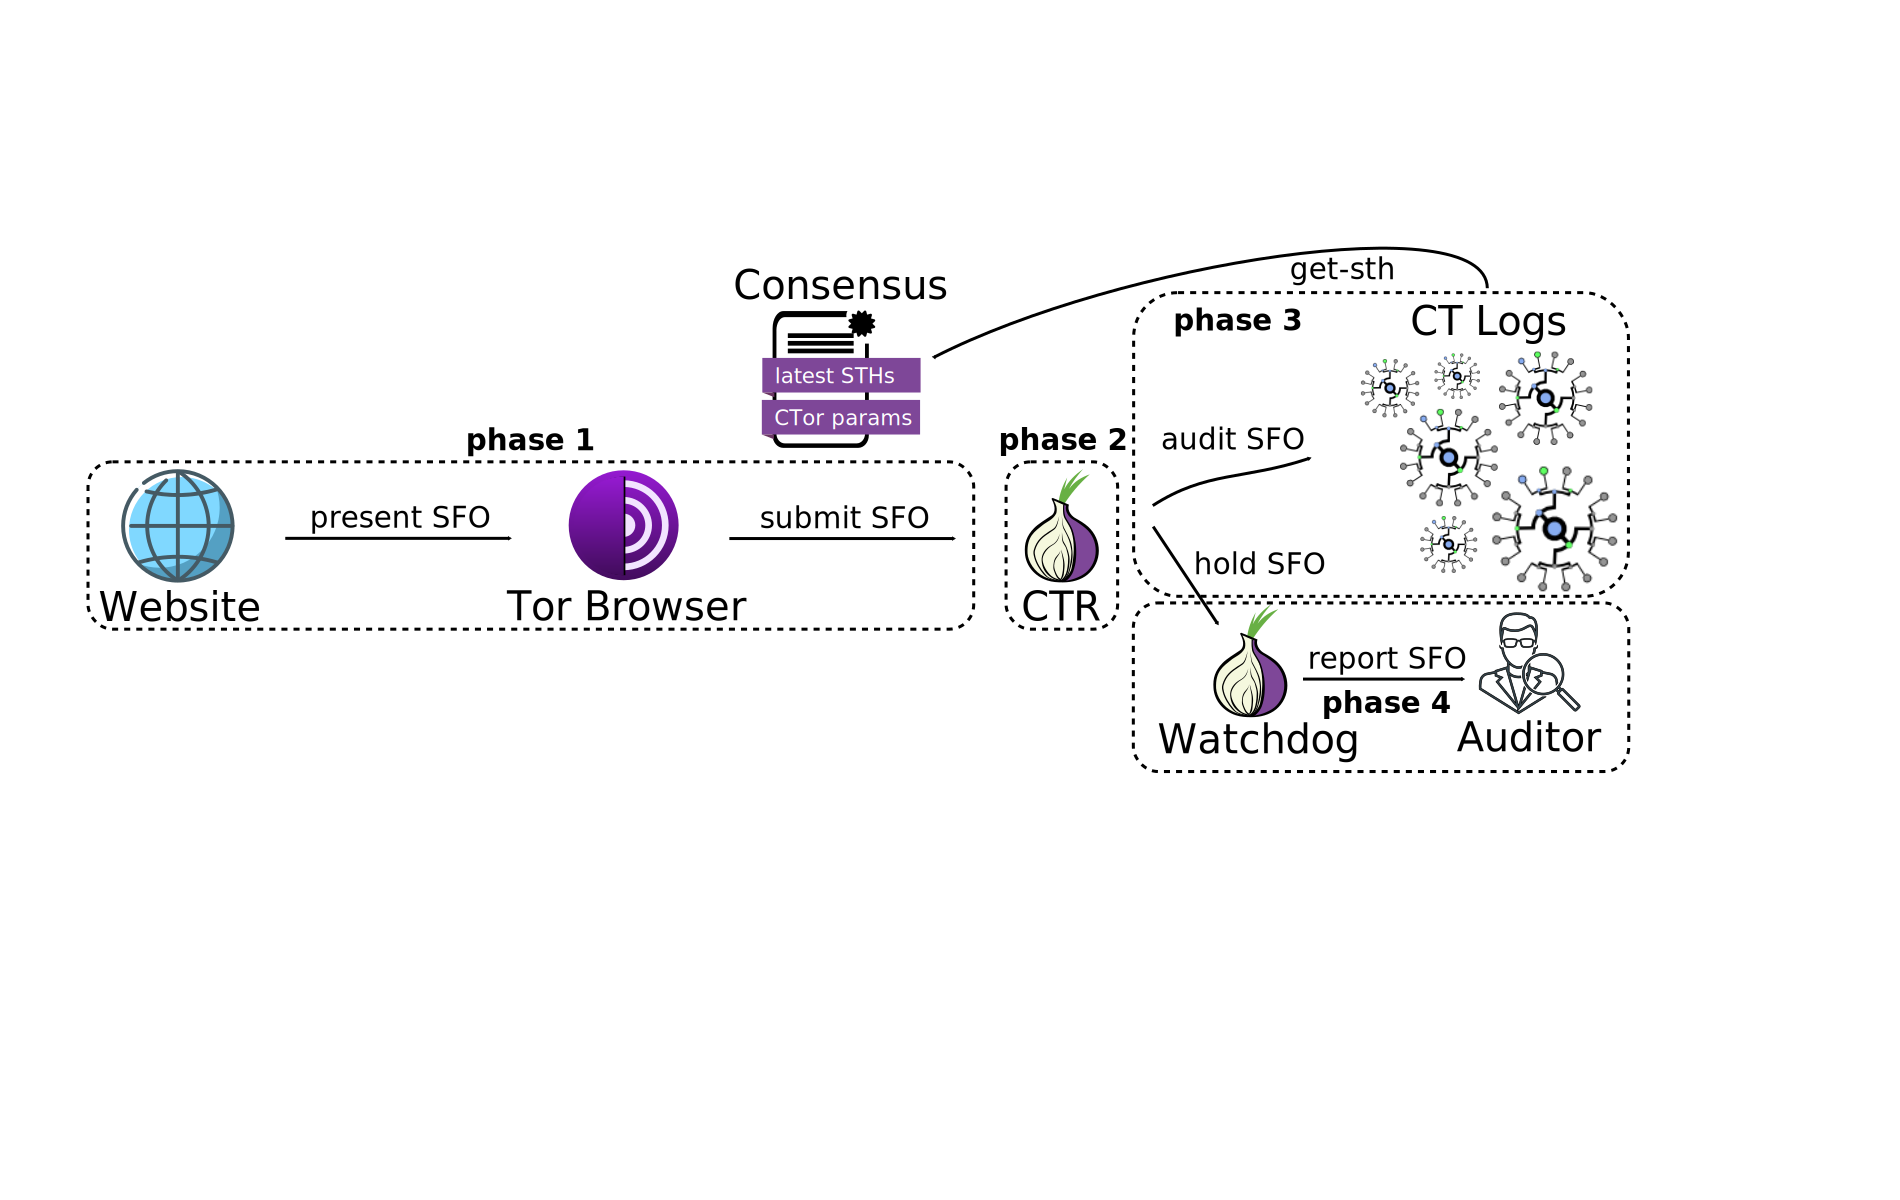
\includegraphics[width=0.8\textwidth]{img/design}
	\vspace{-8px}
	\caption{%
		An overview of the four phases of the full CTor design. In phase 1 Tor
	Browser submits a SFO (SCT Feedback Object) to a Certificate Transparency
	Relay (CTR), followed by phase 2 where the CTR buffers the SFO. In phase 3
	the relays attempts to audit the SFO, and in case of failure, it reports the
	SFO to an auditor with the help of a watchdog CTR in phase 4.}
	\label{fig:design}
	\vspace{-10px}
\end{figure*}

\subsection{Phase~1---Tor Browser} \label{sec:base:phase1}

The least complicated auditing design would be one where Tor Browser receives a
TLS certificate and accompanying SCTs (we will refer to this bundle as an SCT
Feedback Object, or SFO for short) and talks to the corresponding logs, over
Tor, requesting an inclusion proof for each SCT. In an ordinary browser, this
would be an unacceptable privacy leak to the log of browsing behavior associated
with an IP address; performing this request over Tor hides the user's IP address
but still leaks real-time browsing behavior.

An immediate problem with this design is that a primary requirement of Tor
Browser is to persist no data about browsing behavior after the application
exits. If we assume that browsers are not left running for long periods of time,
the inclusion proof request can be easily circumvented by the attacker by using
a fresh SCT whose MMD has not completed---thus no inclusion proof can be
provided by the log as per the CT standard. A second problem is that the STH
returned from any inclusion proof exists in a \emph{trust vacuum}: there is no
way to know that it is consistent with other STHs and not part of a split view.

We can evolve the design by adding two components: a list of STHs that Tor
Browser receives over a trusted channel and the participation of a trusted third
party with the ability to persist data and perform auditing actions at a later
point in time.

A single third party used by all users of Tor Browser would receive a
considerable aggregation of browsing behavior and would need to scale in-line
with the entire Tor network. A small number of auditors presents privacy and
single-point-of-failure concerns. A large number would be ideal but presents
difficulties in curation and independent management and still requires scaling
independent of the Tor network. These concerns do not entirely preclude the
design, but they can be easily avoided by reusing relays in the Tor Network as
our trusted third parties: we call the relays so designated Certificate
Transparency Relays (CTRs).

Now, when the browser is completing the TLS handshake, it simultaneously either
passes the SFO to a CTR (if the MMD of the SCT has not elapsed) or queries the
log itself for an inclusion proof to a trusted STH\@.  However, if we presume
the attacker can serve an exploit to the browser, the latter behavior is
immediately vulnerable. The log, upon receiving an inclusion proof request for
an SCT that it knows is malicious, can delay its response. The TLS connection in
the browser, having succeeded, will progress to the HTTP request and response,
at which point the exploit will be served, and the SFO (containing the
cryptographic evidence of CA and log misbehavior) will be deleted by the exploit
code. While blocking the TLS connection until the CT log responds is an option,
experience related to OCSP hard-fail indicates that this notion is doomed to
fail~\cite{no-hard-fail}.

The final change of the design has Tor Browser submit the SFO to the CTR
immediately upon receipt (with some probability) in all cases. A consequence of
this shift is that the trusted STH list no longer needs to be delivered to the
browser but rather the CTRs. To mitigate the risk of a browser exploit being
able to identify the CTR to the attacker (who could then target it), we prepare
\emph{CTR circuits} ahead of time that are closed and discarded as soon as the
SFO is sent. This allows the SFO submission to race with the TLS connection
completion and HTTP request/response. An added detail is to block the TLS
connection in the case that an SFO is unusually large, as defined by a parameter
\texttt{ct-large-sfo-size}. A large SFO may indicate an attempt to win the race
between SFO submission and exploitation. The parameter can be set such that it
happens extremely rarely on legitimate connections, as shown in
Section~\ref{sec:performance}.

We summarize this phase with the following algorithm that provides more explicit
steps and details, and adds a parameter \texttt{ct-submit-pr} that indicates a
probability that an SFO is submitted to a CTR---this provides probabilistic
security while providing the ability to adjust submission rates to account for
CTR scaling issues. Given an incoming SFO $s$, Tor Browser should:
\begin{enumerate}
    \item Raise a certificate error and stop if the certificate chain of $s$
        is not rooted in Tor Browser's trust store.
    \item Raise a certificate transparency error and stop if the SCTs of $s$
        fail Tor Browser's CT policy.
    \item If $\mathsf{len}(s) < \texttt{ct-large-sfo-size}$, accept $s$ and
        conduct the remaining steps in the background while the TLS connection
        and subsequent HTTP request/response proceed. If $\mathsf{len}(s) \geq
        \texttt{ct-large-sfo-size}$ pause the TLS handshake, complete the
        remaining steps, accept~$s$ as valid and then continue the handshake.
    \item Flip a biased coin based on \texttt{ct-submit-pr} and stop if the
        outcome indicates no further auditing.
    \item Submit $s$ to a random CTR on a pre-built circuit. The circuit used
        for submission is closed immediately without waiting for any
        acknowledgment.
\end{enumerate}

\subsection{Phase 2---Buffering} \label{sec:base:phase2}

Once received, the most straightforward thing for a CTR to do is to contact the
issuing log and request an inclusion proof relative to a trusted STH\@. (And if
the SCT's MMD has not elapsed, hold the SFO until it has.) However, this
proposal has two flaws, the first of which leads us to the design of Phase 2.

Immediately contacting the log about an SFO (a) allows the log to predict when
exactly it will receive a request about an SFO and (b) discloses real-time
browsing behavior to the log. The former problem means that an attacker can
position resources for perpetuating an attack ahead-of-time, as well as letting
it know with certainty whether a connection was audited (based on
\texttt{ct-submit-pr}). The latter is some amount of information leakage that
can help with real-time traffic analysis. 

Because a CTR must support storing SCTs regardless, we can schedule an event in
the future for when each SFO would be sent. Adding a per-SFO value sampled from
\texttt{ct-delay-dist} effectively adds stop-and-go
mixing~\cite{kesdogan:ih1998} to the privacy protection, but where there is only
one mix (CTR) between sender (client) and receiver (CT log). So there is no
point in a client-specified interval-start-time such that the mix drops messages
arriving before then, and there is no additional risk in having the interval end
time set by the mix rather than the sender. This means both that some SFOs a
client sends to a CTR at roughly the same time might be in different batches of
SFOs sent to a CT log and that SFOs submitted to that CTR by other honest
clients are more likely to be mixed with these.


In addition to storing SFOs for mixing effects, we also add a layer of caching
to alleviate stored data {\bf \color{red} Does ``to alleviate stored data'' just
mean ``to reduce the overhead of storing data''?}\\
and unnecessary log connections and data disclosure. So with
regards to some CT circuit, an incoming SFO $s$ is processed as follows:
\begin{enumerate}
    \item\label{enm:storage:close} Close the current circuit to enforce one-time
        usage.
    \item\label{enm:storage:unrecognized} Discard all SCTs in the SFO for logs the
        CTR is not aware of; if no SCTs remain then discard the entire SFO\@.
    \item\label{enm:storage:cached}
        Stop if $s$ is cached (see Section~\ref{sec:base:phase3}) or already
        pending to be audited.
    \item\label{enm:storage:fix-log} Sample a CT log $l$ that issued a
        remaining SCT in~$s$.
    \item\label{enm:storage:audit-after} Compute an \texttt{audit\_after}
		time~$t$, see Figure~\ref{fig:audit-after}.
    \item\label{enm:storage:store} Add $(l,t,s)$ to a buffer of pending SCTs to audit.
\end{enumerate}

Recall from Section~\ref{sec:background:ct} that an inclusion proof is fetched
with regards to an STH\@.  As such, we discard SCTs that cannot be verified due
to lack of a trusted STH\@.  The sampled CT log $l$ now refers to an entity that
issued an SCT in the submitted SFO, and it will be challenged to prove inclusion
in phase~3 sometime after the \texttt{audit\_after} timestamp $t$ elapsed. We
can choose one SCT (and therefore log) at random from the SFO, because it is
sufficient to catch only one misbehaving log so long as we report the entire
SFO, allowing for other malicious logs to be identified. (And if one log is
malicious and others are honest; the honest logs will have ensured publication
of the malicious certificate.)


The \texttt{audit\_after} timestamp specifies the earliest point in time that an
SCT from an SFO will be audited in Phase~3, which adds random noise that
obfuscates real-time browsing patterns in the Tor network and complicates
predictions of when it is safe to assume no audit will take place.  If memory
becomes a scarce resource, pending triplets should be deleted at
random~\cite{nordberg}. Figure~\ref{fig:audit-after} shows that $t$ takes the
log's MMD into account.  This is one of two parts that prevent \emph{early
signals} to the issuing CT logs that an SFO is being audited.  For example, if
an SFO is audited before the MMD elapsed, the issuing CT log could simply merge
the underlying certificate chain to avoid any MMD violation.

% TODO: If we're going to say 'one of two early signals' we need to clearly identify the other one. And it's not clear to me what else specifically is considered such an early signal.

\begin{figure}
	\centering
	\pseudocode[linenumbering, syntaxhighlight=auto]{%
		\textrm{t} \gets \mathsf{now}() +
			\mathsf{MMD} +
			\mathsf{random}(\texttt{ct-delay-dist}) \\
		\pcif \textrm{SCT.timestamp} + \textrm{MMD} <
				\mathsf{now}():\\
			\pcind\textrm{t} \gets \mathsf{now}() +
				\mathsf{random}(\texttt{ct-delay-dist})
	}
	\caption{%
		Algorithm that computes an \texttt{audit\_after} timestamp $t$.
	}
	\label{fig:audit-after}
\end{figure}

\subsection{Phase 3---Auditing} \label{sec:base:phase3}

As alluded to in Phase 2, there is a second problem why the simple behavior of
`contact the log and request an inclusion proof' is unacceptable. We include the
ability to DoS an individual Tor relay in our threat model---if the log knows
which CTR holds the evidence of its misbehavior, it can take the CTR offline,
wiping the evidence of the log's misbehavior from its memory. 

We can address this concern in a few ways. The simple proposal of contacting the
log over a Tor circuit will not suffice---a log can tag each CTR by submitting
unique SFOs to them all, and recognize the CTR when they are submitted. Even
using a unique Tor circuit for each SFO might not suffice to prevent effective
tagging attacks. For example, after tagging all CTRs, a malicious log could
ignore all but innocuous untagged requests and tagged requests matching tags for
whichever CTR it responds to first. If exponential backoff is supported, the
rest of the CTRs will backoff repeated attempts to fetch a proof until the first
CTR has emptied itself of pending SFOs. Then the log can repeat this process
until it receives the offending SFO\@. With high probability this will come in
the midst of a string circuits with tags from a particular CTR (as opposed to
being requested on the first circuit from some CTR). This might result in many
CTRs reporting the log as inaccessible for days, but that is not the same as
direct evidence of misbehavior.

{\bf \color{red} Paul did not understand this
  despite-one-SFO-per-circuit tagging attack as it was written and had
  to write it up differently till he did. I think I've captured the
  attack, which is the most important thing. Let me know.\\ \\
  I still don't see how this is likely to be effective given (a) how long it
  will take CTRs to send all their currently pending SFOs, (b) that the log
  won't be able to tell when a given CTR has finished sending all the SFOs it
  has pending for that log, so OK to move to the next one, (c) the expected
  number of CTRs to run through till the offending SFO pops up (if ever
  depending on coin flips), and (d) with the randomized delay, there is a fair
  chance that the offending SFO won't come up the first time a CTR is the
  current target.\\ \\
  Totally making numbers up: if there are 25 CTRs in the network, and
  it takes an hour to be reasonably sure the current target has run
  through its whole current pending pile, and expected iterations till
  an offending SFO comes up is 2, then many CTRs will have noticed
  the log as unavailable for days. I guess this is a much lesser
  offense and tried to note it, though on top of everything else
  it would seem to make likely that the attack can't be conducted
  more than once or twice since being repeatedly unavailable broadly
  might be an issue.}


While there are ways to detect this attack after-the-fact, and there may be ways
to mitigate it, a more robust design would tolerate the disclosure of a CTRs
identity to the log without allowing a Denial-of-Service attack to erase
evidence of misbehavior.  The simple approach is to write the data to disk prior
to contacting the log; however, Tor relays are explicitly designed not to write
data about user behavior to disk unless debug-level logging is enabled. Relay
operators have expressed an explicit desire to never have any user data
persisted to disk, as it changes the risk profile of their servers with regards
to search, seizure, and forensic analysis.

The evolved design is to have the CTR work with a partner CTR---we call it a
watchdog---whom they choose at random and contact over a Tor circuit. Prior to
talking to a log, the CTR provides the watchdog with the SFO it is about to
submit. After an appropriate response from the log, the CTR tells the watchdog
that SFO has been adequately addressed.

Each CTR maintains a single shared circuit that is used to interact with all CT
logs known to the CTR\@. (We are not using one circuit per SFO given the
overhead and the unclear security benefit noted above.) For \emph{each} such CT
log $l$, the CTR runs the following steps indefinitely:
\begin{enumerate}
    \item\label{enm:auditing:backoff} Sample a delay $d \gets
        \mathsf{random}(\texttt{ct-backoff-dist})$ and wait until $d$ time units
        elapsed.
    \item Connect to a random watchdog CTR\@.
    \item\label{enm:auditing:loop} For each pending buffer entry $(l',s,t)$,
    where $l' = l$ and $t <= \mathsf{now}()$:
		\begin{enumerate}
			\item\label{enm:ext:auditing:watchdog} Share $s$ with the current
				watchdog.
			\item\label{enm:ext:auditing:challenge} Challenge the log to prove
                                  inclusion to a known STH, waiting for
                                  \texttt{ct-log-timeout} before timing out.
				\begin{itemize}
					\item\label{enm:ext:auditing:challenge:success} On valid
						proof: send an acknowledgment to the watchdog, then
						cache $s$ and discard it.
					\item\label{enm:ext:auditing:challenge:fail} On any other
						outcome: discard $s$, close circuit to the watchdog CTR,
						and go to step~1.
				\end{itemize}
		\end{enumerate}
\end{enumerate}

\subsection{Phase 4---Reporting}

At any given time, a CTR may be requesting inclusion proofs from logs (we will
refer to this role as the log-challenger) and may also be a watchdog for one or
more other CTRs. A CTR acting as a watchdog will have at most one SFO held
temporarily for each log-challenger it is interacting with. If a response from
the log-challenger is not received within \texttt{ct-watchdog-timeout}, it
becomes the watchdog's responsibility to raise it for human intervention. This
end-stage process that begins with the watchdog's receipt of a suspicious SFO
and culminates in human review is referred to as auditing, and left
mostly-unspecified.

Because human review and publication\footnote{Most likely on the ct-policy group
at \url{https://groups.google.com/a/chromium.org/forum/\#!forum/ct-policy}} is
critical, we envision that the watchdog (which is a Tor relay that may not be
closely monitored) provides the SFO to an independent auditor run by a human
closely monitoring its operation. When arriving at the design of the CTR being a
role played by a Tor relay, we eschewed separate auditors because of the lack of
automatic scaling with the Tor network, the considerable aggregation of browsing
behavior across the Tor network, and the difficulties of curation and validation
of trustworthy individuals. SFOs submitted to auditors at this stage have been
filtered through the CTR layer, resulting in an exponentially smaller load (and
data exposure) for auditors and allowing a smaller number of them to operate
without needing to scale with the network.

While we consider all auditors trusted---the watchdog needs to take precautions
talking to them because the network is not trusted\footnote{While our threat
model, and Tor's, precludes a global network adversary, we both include partial
network control within the threat model.}. If the watchdog contacted the auditor
without a Tor circuit, an adversary watching the auditors' network connections
could induce a watchdog to contact the auditor, learn the watchdog's identity,
pause their network connection, and perform a Denial of Service attack erasing
the evidence of misbehavior. To mitigate this, the watchdog can contact an
auditor as soon as it receives an SFO it should report; however it must contact
the auditor over a Tor circuit. If a successful acknowledgement from the auditor
is not received within \texttt{ct-auditor-timeout}, the SFO is buffered and
should be re-presented to the same auditor after a random delay.

When an auditor receives an SFO, it should persist it to durable storage until
it can be successfully resolved to a trusted STH\@. Once so persisted, the
auditor can begin querying the log itself asking for an inclusion proof. If no
inclusion proof can be provided after some threshold of time, or the inclusion
proof shows evidence of a MMD violation, the auditor software should raise the
details to a human operator for investigation.

Separately, the auditor should be retrieving the current Tor consensus and
ensuring that a consistency proof can be provided between STHs from the older
consensus and the newer. If consistency can be established, the older STH can be
discarded. If consistency cannot be established after some threshold of time,
the auditor software should raise the details to a human operator for
investigation. It would also be possible for an auditor to monitor a log's
uptime and report on excessive downtime.

\subsection{Additional Details} \label{sec:base:consensus}

\subsubsection{CTR Flag} \label{sec:base:consensus:ctr-flag} Within the Tor
consensus, the existing \texttt{known-flags} item determines the different flags
that the consensus might contain.  We add another flag named \texttt{CTR}, which
indicates that a Tor relay should support CT-auditing as described here. For
now, assume that a relay qualifies as a CTR if it is flagged as \texttt{stable}
and not \texttt{exit}, to spare the relatively sparse exit bandwidth and only
use relays that can be expected to stay online. Section~\ref{sec:privacy}
discusses trade-offs in the assignment of the \texttt{CTR} flag.

\subsubsection{Trusted STHs}
Tor's consensus should capture a fixed view of the CT landscape by publishing
STHs from all recognized logs.  A CT log is recognized if a majority of
directory authorities proposed a \texttt{ct-log-info} item, which contains a
log's ID, public key, base URL, MMD, and most recent STH\@.  Each directory
authority proposes its own STH, and agrees to use the most recent STH as
determined by timestamp and lexicographical order.  Since CTRs verify inclusion
with regards to SCTs that TB accepts, the CT logs recognized by TB must be in
Tor's consensus.

\subsubsection{Trusted Auditors}
Tor's directory authorities also majority-vote on \texttt{ct-auditor} items,
which pin base URLs and public keys of CT auditors that watchdogs contact in
case that any log misbehavior is suspected.  A watchdog triggers if the time
specified by \texttt{ct-watchdog-timeout} elapses without receiving any
acknowledgment.  The following auditor submission is governed by a
\texttt{ct-auditor-timeout}, which, if triggered, results in a resubmission
later on.

\subsubsection{Other Parameters} \label{sec:base:consensus:params} Directory
authorities influence the way in which TB and CTRs behave by voting on other
necessary parameters. Below, the value of an item is computed as the median of
all votes.
\begin{description}
    \item[ct-submit-pr:] A floating-point in $[0,1]$ that determines Tor
        Browser's submission probability.  For example, $0$ disables submissions
        while $0.10$ means that every 10$^{\mathsf{th}}$ SFO is sent to a random
        CTR on average.
    \item[ct-large-sfo-size:] A natural number that determines how many
        wire-bytes a normal SFO should not exceed.  As outlined in
        Section~\ref{sec:base:phase1}, excessively large SFOs are subject to
        stricter verification criteria.
    \item[ct-log-timeout:] A natural number that determines how long a CTR waits
        before concluding that a CT log is unresponsive, e.g., 10~seconds. As
        outlined in Section~\ref{sec:base:phase3}, timeouts trigger implicit
        resubmissions.
    \item[ct-delay-dist:] A distribution that determines how long a CTR should
        wait at minimum before auditing a submitted SFO\@.  As outlined in
        Section~\ref{sec:base:phase2}, random noise is added, e.g., on the order
        of minutes to an hour.
    \item[ct-backoff-dist:]
        A distribution that determines how long a CTR should wait between two
        auditing instances, e.g., a few minutes on average.  As outlined in
        Section~\ref{sec:base:phase3}, CTRs audit pending SFOs in batches at
        random time intervals to spread out log overhead.
    \item[ct-watchdog-timeout]
    \item[ct-auditor-timeout]
\end{description}

  \section{Security Analysis} \label{sec:analysis}
TODO: risk, security of base design

  \section{Incremental Deployment} \label{sec:incremental}
Section~\ref{sec:base} covered a full end-to-end design that places zero-trust
in the CT landscape by challenging the logs to prove certificate inclusion with
regards to trusted STHs in the Tor consensus.  If no such proof can be provided,
the suspected evidence of log misbehavior is reported to a trusted CT auditor
that follows-up on the incident, which involves human intervention if an issue
persists.  The proposed solution modifies the Tor consensus, Tor Relays, and Tor
Browser.  It also requires development and deployment of a new trusted auditor
infrastructure.  The current lack of the latter makes it unlikely that
we will see
adoption of CTor in its full potential anytime soon, and begs the question of
increments that help us get there in the future.  Therefore, we additionally
propose a scaled-down design that can be part of a gradual deployment.

Without the ability to rely on CT auditors, trust needs to be shifted elsewhere
because we cannot expect the average Tor relay operator to continuously persist
and manually investigate SFOs that cannot be resolved.  At the same time, an
incremental proposal that does not improve upon the currently deployed
assumption of pairwise-independently trusted CT logs is not much of a
step forward.
These observations lead us towards
	\emph{collective trust in all CT logs}.
Such an assumption is suboptimal on paper, but it does provide real-world
security improvements by raising the bar towards unnoticed certificate
mis-issuance from weakest-link(s) to quite the opposite.

The smallest change of the full design would be for watchdogs to report
suspected certificate mis-issuance to all CT logs, simply by using the public
\texttt{add-chain} API to make the SFO's certificate chain transparent.  This
has the benefit of holding the CA accountable \emph{if some log operator is
benign}.  Given that our attacker is risk-averse, reporting to a single
independent log\footnote{%
	The independent log need not be trusted by the browser, i.e., it could be
	specified separately in the Tor consensus.  An operator that runs such a
	log would help distribute trust and facilitate auditing.
	Appendix~\ref{app:ct-trust-anchors} provides details on today's log
	ecosystem.
} that issued none of the accompanied SCTs would likely be sufficient.  There is
also room for further simplification.  For example, there is no point in
challenging the logs to prove inclusion if the fallback behavior of no response
only makes the issued certificate public, i.e., not SCTs.
{\bf \color{red} Paul doesn't understand ``i.e., not SCTs''.}
  Thus, CTRs could opt
to cross-log immediately \emph{without ever distinguishing between certificates
that are benign and possibly fraudulent}.  This results in the scaled-down
design shown in Figure~\ref{fig:cross-log}, which initially removes several
system complexities (such as extra-info metrics, auditor infrastructure,
watchdog collaborations, and inclusion proof fetching against trusted STHs in
Tor's consensus).

\begin{figure*}
    \centering
	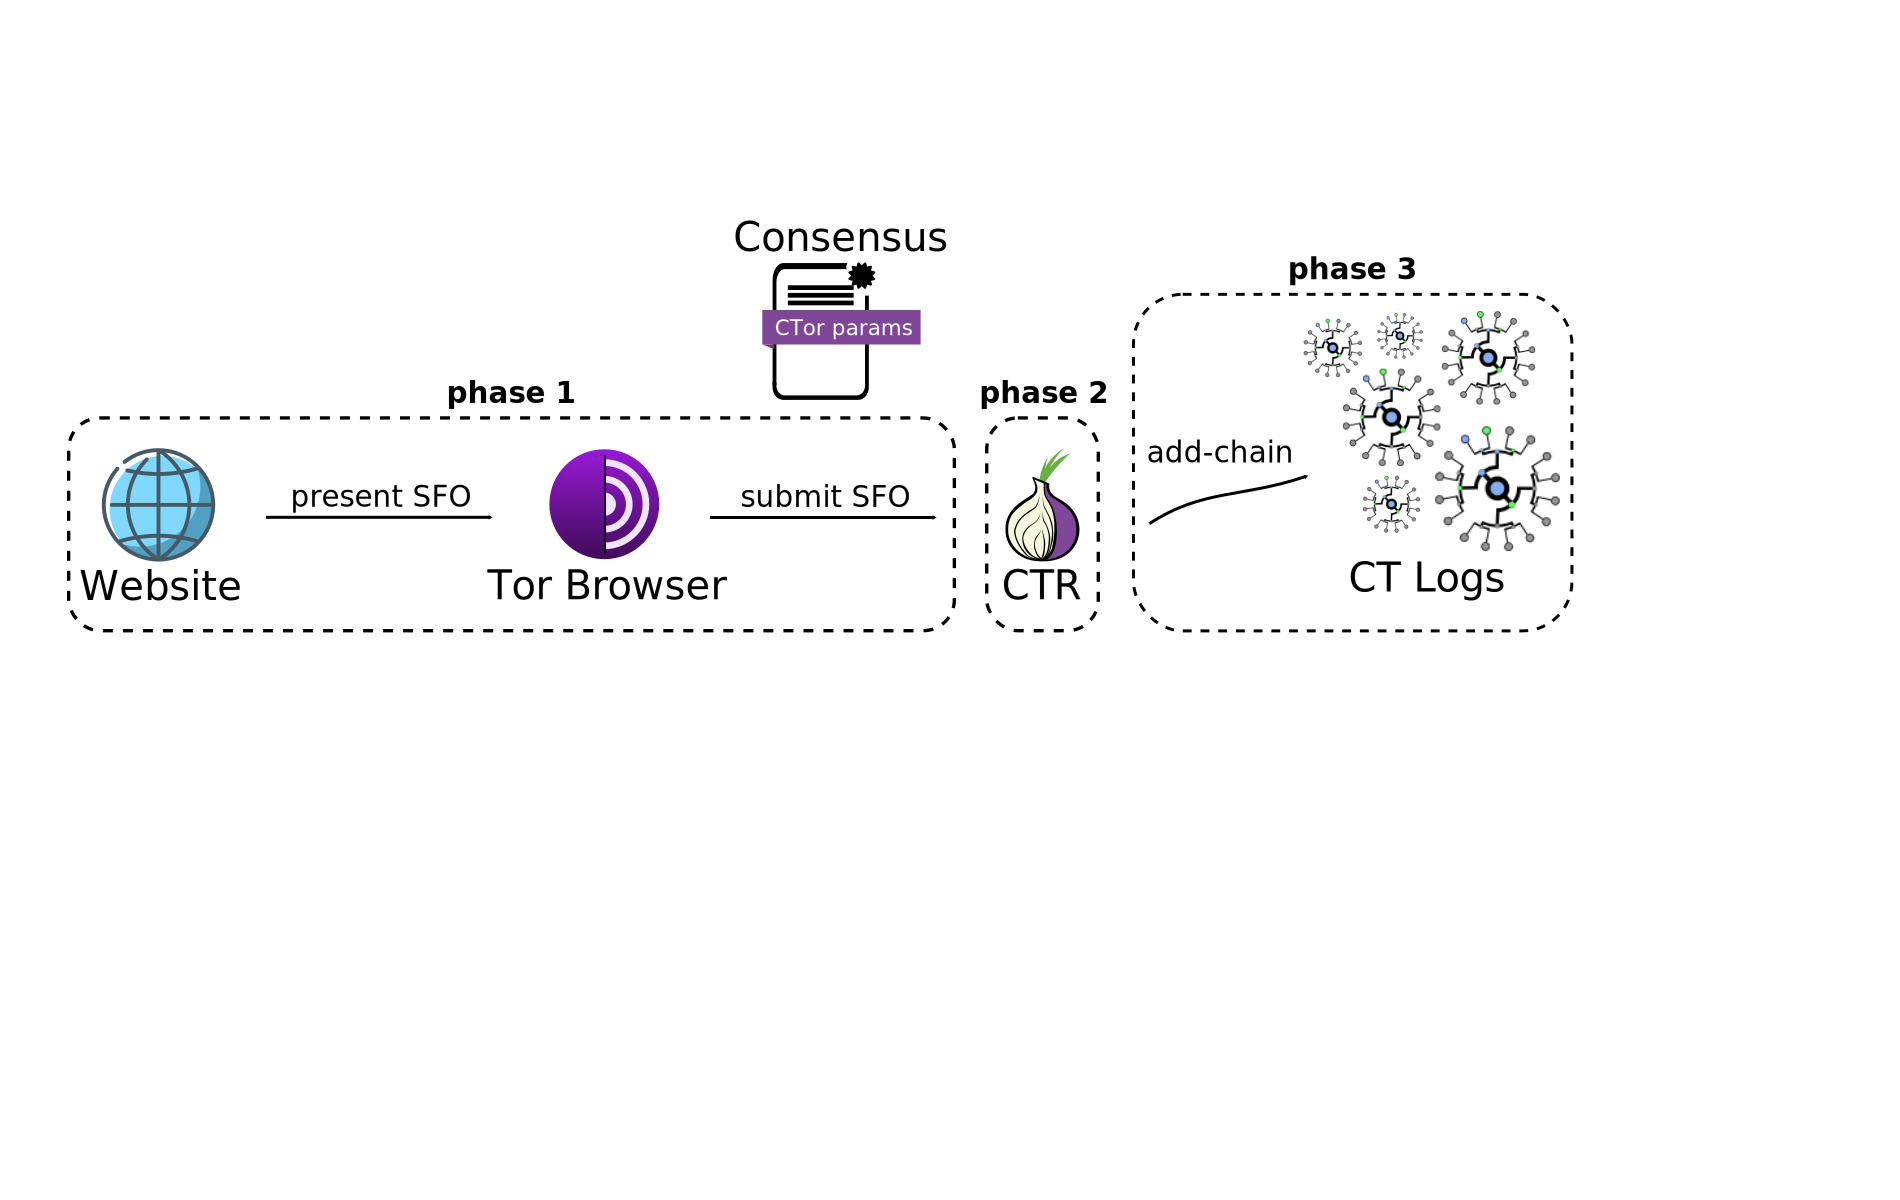
\includegraphics[width=0.8\textwidth]{img/design-ca}
	\vspace{-8px}
	\caption{%
		Scaled-down design that can be deployed incrementally without any
		trusted CT auditors.  Tor Browser still submits SFOs to CTRs on
		independent Tor circuits for the sake of privacy and security.  After
		CTR buffering, the submitted certificates are \emph{cross-logged} by
		adding them to independent CT logs (selected at random) that the
		attacker does not control (inferred from accompanied SCTs).
	}
	\label{fig:cross-log}
	\vspace{-10px}
\end{figure*}

The drawback of certificate cross-logging is that the misbehaving CT logs cannot
be exposed.  There is also a discrepancy between cross-logging and encouraging
the CT landscape to deploy reliable CT auditors.  We therefore suggest a
minimal change to the basic cross-logging design that addresses both of these
concerns.  This change is unfortunately to the API of CT logs and not Tor.  The
proposed change is to allow cross-logging of a certificate's issued SCTs, e.g.,
in the form of an \texttt{add-sfo} API that would replace \texttt{add-chain}
in Figure~\ref{fig:cross-log}.
This means that CTRs could expose both the mis-issued certificate and the logs
that violated their promises of public logging.  At the same time, the
infrastructural part of a CT auditor is built directly into existing
CT logs:
	accepting SFOs that need further investigation.
Such an API would be an ecosystem improvement in itself, providing a
well-defined place to report suspected log misbehavior on-the-fly
\emph{casually}, i.e., without first trying to resolve an SFO for en extended
time period from many different vantage points and then ultimately reporting it
manually on the CT policy mailing list.

\textbf{Security sketch.} 
There are no changes to Phase~1 because cross-logging is instantiated at CTRs.
Phases~3--4 are now merged, such that the encountered certificates are added to
independent CT logs that the attacker does not control.  This means that the
attacker does not learn anything from Phase~3, which motivates why watchdogs are
only needed in the full design.  The other main difference takes place in
Phase~2, during which CTRs buffer SFOs.  The buffer time used to be lengthy due
to taking early signals and MMDs into account, but it is now a moot point as the
logs are not held accountable.  The expected buffer time can therefore be
shortened down to \emph{minutes} that follow only from the randomness in the
\texttt{audit\_after} timestamp, making network-wide flushes impractical while
at the same time reducing the time that a mis-issued certificate stays unnoticed
(a benign log is likely to add an entry before all MMDs elapsed).

The extended cross-logging also aims to expose log misbehavior.  As such, it is
paramount that no cross-logged SFO becomes public before the issuing CT logs
can merge the mis-issued certificate reactively to avoid catastrophic impact.
This could be assured by buffering newly issued SFOs longer as in the full
design, which brings back the threat and complexity of minor impact scenarios.
Another option that is appealing for Tor (but less so for CT) is to operate the
\texttt{add-sfo} API with the expectation of \emph{delayed merges} that account
for MMDs before making an SFO public, effectively moving lengthy buffering from
CTRs to CT logs with persistent storage.

  %
% emph focus on normal-case behavior, and use distributions that mean auditing
% delay is avg ~10m.  Risk averse attacker would still need to assume shorter
% storage, i.e., success 50\% not enough.
%
\section{Performance} \label{sec:performance}
The following analysis shows that CTor's overhead is modest based on computing
performance estimates from concrete parameter properties and two public data
sets.

\subsection{Setup}
Mani~\emph{et~al.} derived a distribution of website visits over Tor and an
estimation of the number of circuits through the network~\cite{mani}.  We use
their results to reason about overhead as the Tor network is under heavy load,
assuming 140~million daily website visits (the upper bound of a 95\% confidence
interval).  Our analysis also requires a distribution that captures typical SFO
properties per website visit.  Therefore, we collected an SFO data set by
browsing the most popular webpages submitted to Reddit (r/frontpage, all time)
on December 4, 2019.  The parsed data set contains 8858 data points, each of
which correspond to the encountered SFOs.  It is available online as an open
access artifact together with the associated scripts.  Note that browsing
web\emph{pages} as opposed to front-pages (such as Alexa's list) yielded more
SFOs per website visit (we measured), making it less likely that our analysis is
an underestimate.

We found that an average certificate chain is 5440~bytes, and it is seldom
accompanied by more than a few SCTs.  As such, a typical SFO is in the order of
6~KiB.  No certificate chain exceeded 20~KiB, and the average number of SFOs per
webpage was seven.  The latter includes 1--2 SFOs per data point that followed
from our client software calling home on start-up (Chromium~77).

We assume no abnormal CTor behavior, which means that there will be little or
no CTR back-offs due to the high uptime requirements of today's CT logs: 99\%.
We set \texttt{ct-large-sfo-size} conservatively to avoid blocking in the TLS
handshake (e.g., 20~KiB), and use a 10\% submission probability as well as a
10~minute random buffer delay on average.  It is likely unwarranted to use a
higher submission probability given that the intended attacker is risk-averse.
Shorter buffer times would leak finer-grained browsing patterns to the logs,
while longer ones increase the attack surface in phase~2.  Therefore, we
selected an average for \texttt{ct-delay-dist} that satisfies none of the two
extremes.  The remaining CTor parameters are timeouts, which have little or no
performance impact if set conservatively (few seconds).

\subsection{Estimates}
The incremental cross-logging designs are analyzed first without any caching.
Caching is then considered, followed by overhead that appears only in the full
design.

\textbf{Circuit overhead.}
Equation~\ref{eq:sub-oh} shows the expected circuit overhead from Tor Browser
over time, where $p$ is the submit probability and $\bar{d}$ the average number
of SFOs per website visit.  The involved overhead is linear as either of the two
parameters are tuned up or down.

\begin{equation} \label{eq:sub-oh}
	p\bar{d}
\end{equation}

Using $p\gets\frac{1}{10}$ and our approximated SFO distribution $\bar{d}\gets7$
yields an average circuit overhead of $0.70$, i.e., for every three Tor Browser
circuits CTor adds another two.  Such an increase might sound
daunting at first, but these additional circuits are short-lived and
light-weight; transporting 6~KiB on average.  Each CTR also maintains a 
long-lived circuit for CT log interactions.

\textbf{Bandwidth overhead.}  Equation~\ref{eq:bw} shows the expected
bandwidth overhead for the Tor network over time, where
	$V$ is the number of website visits per time unit,
	$p$ the submit probability,
	$\bar{d}$ the average number of SFOs per website visit, and
	$\bar{s}$ the average SFO byte-size.

\begin{equation} \label{eq:bw}
	6Vp\bar{d}\bar{s}
\end{equation}

$Vp\bar{d}$ is the average number of SFO submissions per time unit, which can be
converted to bandwidth by weighting each submission with the size of
a typical SFO and accounting for it being relayed six times:
	three hops from Tor Browser to a CTR, then
	another three hops from the CTR to a CT log.\footnote{%
		Assuming that a Tor relay's available bandwidth is symmetric.
	}
Using
	$V\gets 140\textrm{~M/day}$,
	$p \gets \frac{1}{10}$,
	$\bar{d} \gets 7$,
	$\bar{s} \gets 6\textrm{~KiB}$
and converting the result to bps yields 334.5~Mbps in total.  Such order of
overhead is small when compared to Tor's capacity:
450~Gbps~\cite{tor-bandwidth}.

\textbf{Memory overhead.}
Equation~\ref{eq:memory} shows the expected buffering overhead, where
	$V_m$ is the number of website visits per minute,
	$t$ the average buffer time in minutes,
	$R$ the number of Tor relays that qualify as CTRs, and
	$\bar{s}$ the typical SFO size in bytes.

\begin{equation} \label{eq:memory}
	\frac{V_mt}{R} \bar{s}
\end{equation}

$V_mt$ represent incoming SFO submissions during the average buffer time, which
are randomly distributed across $R$ CTRs.  Combined this yields the expected
number of SFOs that await at a single CTR in Phase~2, and by taking the
byte-size of these SFOs into account we get an estimate of the resulting memory
overhead.  Using
	$V_m \gets \frac{140\textrm{~M}}{24\cdot60}$,
	$t \gets 10$~m,
	$R \gets 4000$ based on the CTR criteria in
		Section~\ref{sec:base:consensus}, and
	$\bar{s} \gets 6\textrm{~KiB}$
yields 1.42~MiB.  Such order of overhead is small when compared to the
recommended relay configuration:
	at least 512~MiB~\cite{relay-config}.

A cache of processed SFOs reduces the CTR's buffering memory and log
interactions proportionally to the cache hit ratio.  Mani~\emph{et al.} showed
that about one third of all website visits over Tor can be attributed to Alexa's
top-1k, and another one third to the top-1M~\cite{mani}.\footnote{%
	Assuming the overrepresented
	\texttt{torproject.org} is removed.
} If we assume 32~byte cryptographic hashes and seven SFOs per website visit,
a cache hit ratio of $\frac{1}{3}$ could be achieved by a 256~KiB LFU/LRU cache
that eventually captures Alexa's top-1k.  Given that the cache requires
memory as well, this is best viewed as a bandwidth optimization.

\textbf{Full design.}
For each CTR and CT log pair, there is an additional watchdog circuit that
transports the full SFO upfront before fetching an inclusion proof.  The
expected bandwidth overhead is at most $9Vp\bar{d}\bar{s}$, i.e., now
also accounting for the three additional hops that an SFO is subject to.  In
practise the overhead is slightly less, because an inclusion query and its
returned proof is smaller than an SFO.  We expect little or no
watchdog-to-auditor overhead if the logs are available, and otherwise one
light-weight circuit that reports a single SFO for each CTR that goes into
back-off.  Such overhead is small when compared to all Tor Browser submissions.
Finally, the required memory increases because newly issued SFOs are buffered
for at least an MMD.  Only a small portion of SFOs are newly issued, however:
	the short-lived certificates of Let's Encrypt are valid for
	90~days~\cite{le}, which is in contrast to 24~hour
	MMDs~\cite{google-log-policy}.


  \section{Privacy} \label{sec:privacy}
There is an inherent privacy problem in the setting due to how CT is designed
and deployed. A browser, like TB, that wishes to validate that SFOs presented to
it are \emph{consistent} and \emph{included} in CT logs must directly or
indirectly interact with CT logs wrt. its observed SFOs. Without protections
like Private Information Retrieval~\cite{PIR} that require server-side support
or introduction of additional parties and trust
assumptions~\cite{lueks-and-goldberg,kales}, exposing SFOs to any party risks
leaking (partial) information about the browsing activities of the user.

Given the constraints of the existing CT ecosystem, CTor is made
privacy-preserving thanks to the distributed nature of Tor with its anonymity
properties and high-uptime relays that make up the Tor network. First, all
communication between TB, CTRs, CT logs, and auditors are made over full
Tor-circuits. This is a significant privacy-gain, not available, e.g., to
browsers like Chrome that in their communications would reveal their public
IPv4-address (among a number of other potentially identifying metadata).
Secondly, the use of CTRs as intermediaries probabilistically delays the
interaction with the CT logs---making correlating TB user browsing with CT log
interaction harder for attackers---and safely maintains a dynamic cache of the
most commonly already verified SFOs. While regular browsers like Chrome could
maintain a cache, TB's security and privacy goals (see
Section~\ref{sec:background:tor}) prohibit such shared (persisted) dynamic
state.

CTRs are also essential for security in the setting of the auditor extension. A
rational attacker will produce SFOs with SCT timestamps that are too new to have
to be part of CT logs at the time of the attack. TB cannot store SFOs for any
extended time period without violating its security and privacy goals, not to
mention that presumably most TB sessions are not maintained for
days (as required, see analysis in Section~\ref{sec:auditor:analysis}) 
{\bf \color{red} What analysis is this pointing at?}\\
but rather minutes~\cite{DBLP:conf/pam/AmannS16}. Further, buffering
at TB is not an option, since an attacker could compromise TB shortly
after presenting the forged SFO.

The main limitation of CTor in terms of privacy is that CTor continuously leaks
to CT logs---and to a \emph{lesser extent} auditors (depending on design)--a
fraction of certificates of websites visited using TB to those that operate CT
logs. This provides to a CT log a partial list of websites visited via the Tor
network over a period of time (determined by \texttt{ct-delay-dist}), together
with some indication of distribution based on the number of active CTRs. It does
not, however, provide even pseudonymously any information about which sites
individual users visit, much less with which patterns or timing. As such it
leaks significantly less information than does OCSP validation by TB or DNS
resolution at exit-relays~\cite{TorDNS}, both of which indicate visit activity
in real time to a comparably small number of entities.

Another significant privacy limitation is that relays with the CTR flag learn
real-time browser behavior of Tor users. Relays without the Exit flag primarily
only transport encrypted Tor-traffic between clients and other relays, never to
destinations. If such relays are given the CTR flag---as we stated in the full
design, see Section~\ref{sec:base:consensus:ctr-flag}---then this might
discourage some from running Tor relays unless it is possible to opt out.
Another option is to give the CTR flag only to exit relays, but this \emph{might
be} undesirable for overall network performance despite the modest overhead of
CTor (Section~\ref{sec:performance}). Depending on the health of the network
and the exact incremental deployment of CTor, there are different trade-offs.
For example, fewer CTRs with higher bandwidth and less memory combined make it
easier to perform flooding attacks that flush the entire network.

  %Paul: mixing?
% cite does-ct-break-the-web somewhere as motivation of TB's SCT CT policy
\section{Related Work} \label{sec:related}
Google's Chrome and Apple's Safari enforce CT by mandating that every TLS
certificate must be accompanied by two independent
SCTs~\cite{chrome-policy,safari-policy}.  We proposed that Tor Browser should
follow suit, but, unlike any other web browser that enforces CT, CTor provides
\emph{concrete next steps} that relax the centralized trust which is otherwise
and evidently misplaced in CT logs~\cite{%
	izenpe-disqualified,%
	venafi-disqualified,%
	gdca1-omission,%
	digicert-log-compromised%
}.

%%%
% Privacy preserving inclusion proofs
%%%
Laurie proposed that inclusion proofs could be fetched over DNS to avoid
additional privacy leaks, i.e., a user's browsing patterns are already exposed
to the DNS resolver but not the logs in the CT landscape~\cite{ct-over-dns}.
CT/bis provides the option of serving stapled inclusion proofs as part of the
TLS handshake in an extension, an OCSP response, or the certificate
itself~\cite{ct/bis}.
Lueks and Goldberg proposed that a separate database of inclusion proofs could
be maintained that supports information-theoretic PIR~\cite{lueks-and-goldberg}.
Kales~\emph{et~al.} improved scalability by reducing the size of each entry
in the PIR database at the cost of transforming logs into multi-tier Merkle
trees, and additionally, showed how the upper tier could be expressed as
a two-server computational PIR database to ensure that any inclusion proof can
be computed privately on-the-fly~\cite{kales}.
Nordberg~\emph{et~al.} avoid inclusion proof fetching by hanging on to presented
SFOs, handing them back to the same origin at a later time~\cite{nordberg}.
In contrast, CTor protects the user's privacy without any persited browser state
by submitting SFOs on independent Tor circuits to CTRs, which in turn add random
noise before there is any log interaction to speak of.  The use of CTRs
enable caching similar to CT-over-DNS, but it does not put the logs in the dark
like PIR could.

%%%
% The same consistent view
%%%
Inclusion proofs are only meaningful if everyone observes the same consistent
STHs.
One option is to configure client software with a list of entities that they
should gossip with, e.g., CT monitors~\cite{chase}, or,
browser vendors could push a verified view~\cite{sth-push}.
Such trusted auditor relationships may work for some but not
others~\cite{nordberg}.
Chuat~\emph{et~al.} proposed that HTTPS clients and HTTPS servers could pool
STHs and consistency proofs which are gossiped on website visits~\cite{chuat}.
Nordberg~\emph{et~al.} suggested a similar variant, reducing the risk of user
tracking by pooling fewer and recent STHs~\cite{nordberg}.
Dahlberg~\emph{et~al.} noted that such privacy-insensitive STHs need not be
encrypted, which could enable network operators to use programmable data planes
to provide gossip as-a-service~\cite{dahlberg}.
Syta~\emph{et~al.} proposed an alternative to reactive gossip mechanisms by
showing how an STH can be cosigned efficiently by many independent
witnesses~\cite{syta}.
A scaled-down version of witness cosigning could be instantiated by
cross-logging STHs in other CT logs~\cite{minimal-gossip},
or, in other append-only ledgers~\cite{catena}.
CTor's extended design in Section~\ref{sec:auditor} ensures that anyone
connected to the Tor network is on the same view by making STHs public in the
Tor consensus.  In contrast, the base design is not about catching log
misbehavior, and the extended design in Section~\ref{sec:log} exposes logs
that misbehave \emph{without} fetching inclusion proofs.

Nordberg proposed that Tor clients could enforce public logging of consensus
documents and votes~\cite{consensus-transparency}.  Such an initiative is
mostly orthogonal to CTor, as it strenghtens the assumption of a secure Tor
consensus by enabling detection of compromised signing keys rather than
mis-issued TLS certificates.  Winter~\emph{et~al.} proposed that Tor Browser
could check self-signed TLS certificates for extact matches on independent Tor
circuits.  Alicherry~\emph{et~al.} proposed that any web browser could
double-check TLS certificates on first encounter using alternative paths and
Tor, again, looking for certificate mismatches and generating warnings of
possible man-in-the-middle attacks~\cite{doublecheck}.  The submission phase in
CTor is similar to such double-checking, expect that there is no normal-case TLS
handshake blocking, browser warnings, or strict assumptions regarding the
attacker's location.

  \section{Conclusion} \label{sec:conclusion}
CTor consists of a base design and two possible extensions with the goal of
adding incremental and privacy-preserving support for Certificate Transparency
to Tor. The use of relays in the Tor network distributes caching of observed
SFOs and delays interactions with CT logs, central to both overall security and
preserving privacy of Tor users. Our analysis also shows that these relays are
the weakest link: the most promising chance of avoiding exposure of compromising
SFOs appears to be to attempt to perform network-wide DoS on relays, or attack
CT logs directly. 

Mitigation of network-wide attacks take us outside of Tor's---and therefore also
our---threat model. That said, we cannot ignore such attacks given the strong
attacker we consider (to some degree in control of both a trusted CA and CT
logs). Several parameters of our design enables Tor to \emph{adapt} to observed
interference with CTor, such as a network-wide DoS of relays, reported targeted
attacks of CT logs, or relays reporting suspected flooding through the
\texttt{ct-delete-bytes}  extra-info. When it comes to TB, the submission
probability (\texttt{ct-submit-pr}) and SFO size threshold
(\texttt{ct-max-sfo-bytes}) could be set such as to force all SFOs to be sent to
a CTR before accepting any new HTTPS application-layer data. During the storage
phase, the consensus specifies each CT log's MMD and the delay distribution
(\texttt{ct-delay-dist}), which can be set to either minimize or maximize the
delay between TB user and CT log interaction. Similarly, trusted auditors
(auditor extension) and log operator relationships (base design and log
extension) are also defined in the consensus and can be tweaked.

Deploying CTor, in particular with the log extension that requires trusted
auditors, would be a significant operational burden. Overall Tor network health
would have to include considerations of tweaking CTor parameters to adapt to
strong attackers. However, the potential gains are significant. Tor users would
benefit from the significant security improvement provided by CT logs. Perhaps
more significantly, Tor would be a system for maintaining a
probabilistically-audited cryptographically-verifiable view of the entire CT log
ecosystem available from Tor’s consensus. This would benefit the wider web and
Internet, since the view from Tor's consensus could serve as a base of trust,
relaxing the necessary trust that currently has to be placed on CT log
operators. As a starting point, our base design turns Tor Browser into a helpful
participant in addressing the weakest-link issue of the CA ecosystem, in line
with the goals of CT.


  %\section*{Acknowledgements}

  \bibliographystyle{abbrv}
  \bibliography{src/ref}

  \appendix
  \section{Detailed Consensus Parameters} \label{app:consensus-params} 

Below, the value of an item is computed as the median of all votes.
\begin{description}
    \item[ct-submit-pr:] A floating-point in $[0,1]$ that determines Tor
        Browser's submission probability.  For example, $0$ disables submissions
        while $0.10$ means that every 10$^{\mathsf{th}}$ SFO is sent to a random
        CTR on average.
    \item[ct-large-sfo-size:] A natural number that determines how many
        wire-bytes a normal SFO should not exceed.  As outlined in
        Section~\ref{sec:base:phase1}, excessively large SFOs are subject to
        stricter verification criteria.
    \item[ct-log-timeout:] A natural number that determines how long a CTR waits
        before concluding that a CT log is unresponsive, e.g., 10~seconds. As
        outlined in Section~\ref{sec:base:phase3}, a timeout causes the watchdog
        to send a SFO to the auditor.
    \item[ct-delay-dist:] A distribution that determines how long a CTR should
        wait at minimum before auditing a submitted SFO\@.  As outlined in
        Section~\ref{sec:base:phase2}, random noise is added, e.g., on the order
        of minutes to an hour.
    \item[ct-backoff-dist:]
        A distribution that determines how long a CTR should wait between two
        auditing instances, e.g., a few minutes on average.  As outlined in
        Section~\ref{sec:base:phase3}, CTRs audit pending SFOs in batches at
        random time intervals to spread out log overhead.
    \item[ct-watchdog-timeout:] A natural number that determines how long time
    at most a watchdog waits before considering a SFO for reporting. Prevents
    the watchdog from having to wait for a circuit timeout caused by an
    unresponsive CTR. Should be set with \texttt{ct-backoff-dist} in mind.
    \item[ct-auditor-timeout] A natural number that determines how long time at
    most a watchdog waits for an auditor to acknowledge the submission of a SFO.
\end{description}

\section{Log Operators \& Trust Anchors} \label{app:ct-trust-anchors}
The standardized CT protocol suggests that a log's trust anchors should
``usefully be the union of root certificates trusted by major browser
vendors''~\cite{ct,ct/bis}.  Apple further claims that a log in their CT program
``must trust all root CA certificates included in Apple's trust
store''~\cite{apple-log-policy}.  This bodes well for CTor:
	we assumed that the existence of independent log operators implies the
	ability to at least add certificate chains (Section~\ref{sec:base}) and
	possibly complete SFOs (Section~\ref{sec:log}) into logs that the attacker
	does not control.
Google's CT policy currently qualifies 31 logs that are hosted by
	Cloudflare,
	DigiCert,
	Google,
	Let's Encrypt, and
	Sectigo~\cite{google-log-policy}.
No log accepts all roots, but the overlap between root certificates that are
trusted by major browser vendors and CT logs increased over
time~\cite{ct-root-landscape}.  Despite relatively few independent log
operators and an incomplete root coverage, the basic and extended
cross-logging in CTor still provides value:
\begin{itemize}
	\item Even if there are no independent logs available for a certificate
		issued by some CA, adding it again \emph{to the same logs} come with
		practical security gains.  For example, if the attacker gained access to
		the secret signing keys but not the actual log infrastructures the
		mis-issued certificate trivially makes it into the public.  If the full
		SFO is added, the log operators could also notice that they were
		compromised.
	\item Most log operators only exclude a small fraction of widely accepted
		root certificates: 1--5\%~\cite{ct-root-landscape}.  This narrows down
		the possible CAs that the attacker must control by 1--2 orders of
		magnitude.  In other words, to be entirely sure that CTor would (re)add
		a mis-issued SFO to the attacker-controlled CT logs, this smaller group
		of CAs must issue the underlying certificate.  It is likely harder to
		take control of Let's Encrypt which some logs and operators exclude due
		to the sheer volume of issued certificates than, say, a smaller CA that
		law enforcement may coerce.
\end{itemize}

Browser-qualified or not, the availability of independent logs that accept the
commonly accepted root certificates provides significant ecosystem value.
Log misbehavior is mostly reported through the CT policy mailing list.  Thus, it
requires manual intervention.  Wide support of certificate chain and SCT
cross-logging allows anyone to \emph{casually} disclose suspected log
misbehavior on-the-fly.

% \section{Trusted Auditor} \label{app:auditor}
% An trusted auditor is expected to accept SFOs at a dedicated endpoint,
% endeavoring to validate the inclusion status of each SCT with regards to the
% first STH in the Tor consensus that elapsed the log's MMD.  If a log appears to
% function correctly except for some evidence that cannot be
% resolved despite multiple attempts that span a given time period, it is
% paramount that the auditor software alerts its operator who can investigate
% the issue further before submitting a full report to the CT-policy mailing list.
% Cases of misbehavior, in detail:
% \begin{itemize}
% 	\item If the log fails to provide a valid inclusion proof for an SCT with
% 		regards to the first applicable STH in the Tor consensus
% 		(certificate omission).
% 	\item If the log fails to provide a valid consistency proof between two
% 		STHs in the Tor consensus
% 		(split-view).
% 	\item If a published STH is future-dated or backdated more than an MMD
% 		(general log misbehavior).
% 	\item If a log ignores some CTRs (uptime misbehavior).
% \end{itemize}

% An unresponsive log can be suspected by observing the watchdog report frequency,
% and possibly confirmed by querying the log in question from different vantage
% points.  Among other extra-info metrics that go beyond received and deleted
% SFO-bytes that the announced CT auditors should check, it could be valuable to
% publish the extent to which CTR-to-log interactions fail.

% While not within our threat model, we do encourage that the announced auditors
% verify whether STHs in the Tor consensus are consistent with external views of
% the CT landscape.  For example, operate an STH pollination
% endpoint~\cite{nordberg} and fetch STHs actively from many diverse vantage
% points using Tor, VPN services, DoH resolvers, and RIPE Atlas (to mention a few
% options).  This goes back to the point of general ecosystem value.

\section{Flushing a Single CTR} \label{app:flush}
Let $n$ be the number of SFOs that a CTR can store in its buffer.  The
probability to sample a target SFO is thus $\frac{1}{n}$, and the probability to
not sample a target SFO is $q = 1 - \frac{1}{n}$.  The probability to not sample
a target SFO after $k$ submissions is $q^k$.  Thus, the probability to sample
the relevant buffer index at least once is $p = 1 - q^k$.  Solving for $k$ we
get: $k = \frac{\log(1 - p)}{\log(q)}$.  Substituting $q$ for $1 - \frac{1}{n}$
yields Equation~\ref{eq:flush}, which can be used to compute the number of
SFO submissions that the attacker needs to flush a buffer of $n>2$
entries with some probability~$p\in[0,1)$.

\begin{equation} \label{eq:flush}
	k = \frac{\log(1-p)}{\log(1 - \frac{1}{n})}
\end{equation}

It is recommended that a non-exit relay should have at least 512MB of memory.
If the available bandwidth exceeds 40Mbps, it should have at least
1GB~\cite{relay-config}.  Given that these recommendations are lower bounds,
suppose the average memory available to store SFOs is 1GiB.
Section~\ref{sec:performance} further showed that the average SFO size is
roughly 6KiB.  This means that the buffer capacity is $n \gets 174763$ SFOs.
Plugging it into Equation~\ref{eq:flush} for $p \gets \frac{9}{10}$, the
attacker's flood must involve $k \gets 402406$ submissions.  In other words,
2.3GiB must be transmitted to flush a single CTR with 90\% success probability.

As a corner case and implementation detail, it is important that Tor Browser and
CTRs \emph{reject} SFOs that are bogus in terms of size: it is a trivial DoS
vector to load data indefinitely. Analysis based on, e.g., 1~MiB SFOs also
requires 2.3~GiB of data to flush, however.

\end{document}
